% !TEX root = UAV_Landing_Pad.tex
\chapter{Design  and Implementation}\label{chapterDesignAndImplementation}

This section is used to describe the design details for each of the major components 
in the system.  As the construction of an automated UAV/ UGV can be broken into the
common underlying software components and the separable physical and software
differences at each level, this section will be thus divided.  In the first section we overview
the software, starting with the overall architecture of the system in Section~\ref{softwarecustomapi}, and then delving into the various focused components of the project in Sections~\ref{softwarecraftorientation} through~\ref{softwarecontrolpanel}.  Section~\ref{uav} details the design and construction of the Unmanned Aerial Vehicle, and Section~\ref{ugv} details the design and construction of the Unmanned Ground Vehicle.
 

\section{Software: Custom API}\label{softwarecustomapi}

\subsection{Technologies  Used}
The Custom API itself is written in C with the ROS libraries integrated for passing ROS messages. However, the API is designed to handle and interface with the various other technologies used in the landing pad project. The following components that work with the API are listed in the Component Overview.

\subsection{Component  Overview}
\begin{itemize}
  \item Linux OS
  \item gcc
  \item python
  \item R.O.S.
  \item OpenCV
  \item SLAM (HectorSLAM, LSDSLAM, PTAM)
\end{itemize}

\subsection{Phase Overview}
The modular design of ROS made the software environment a sensible choice for our project which incorporates the use of 

While it was the focus of this project to use mostly existing architectures to bring
about the functionality of UAV and UGV, variability was discovered within the 
connectivity of these components.  As such a custom API was implemented to
facilitate the building of custom new functionality and simplify the communication
between custom built software and existing code.

\subsection{ Architecture  Diagram}
Figure~\ref{apinode} details the architecture of the Custom API and demonstrates how it is used to facilitate communication amongst the various components in the software architecture.

\begin{figure}[tbh]
\begin{center}
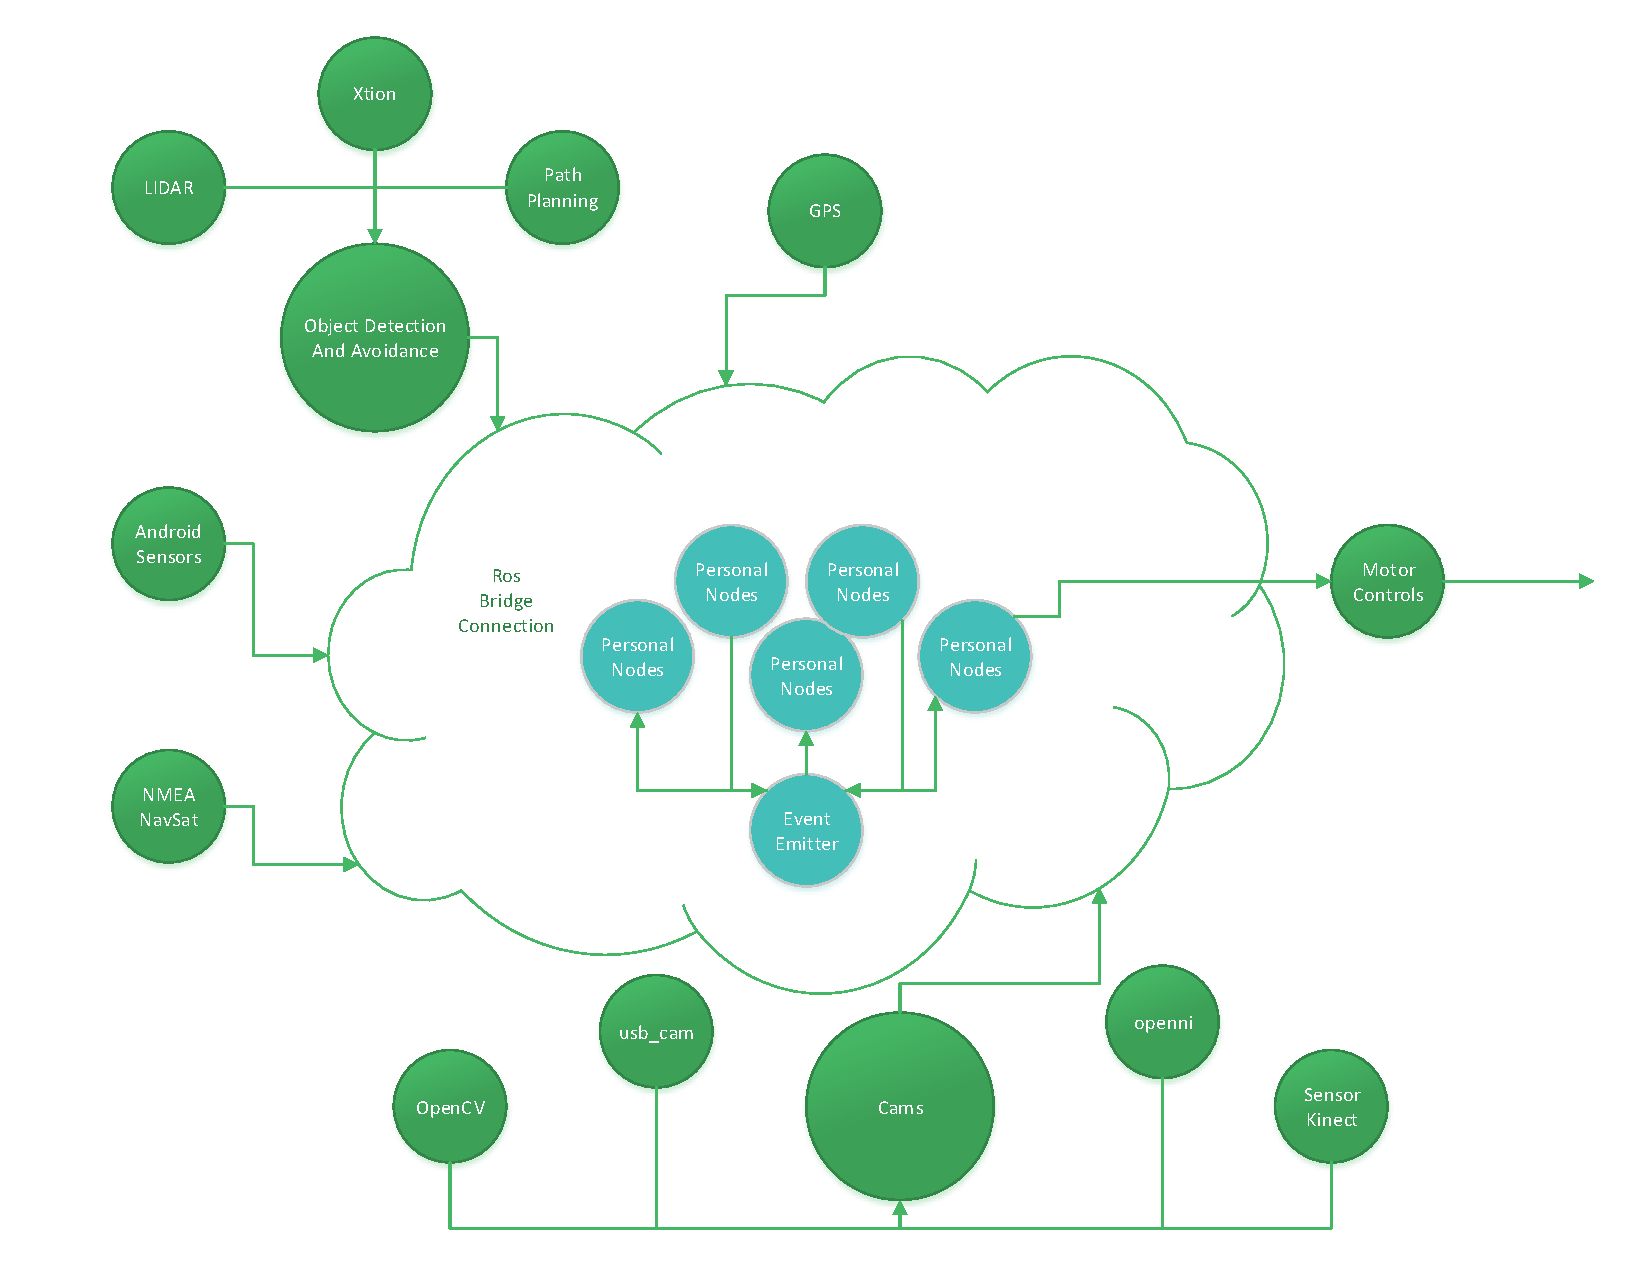
\includegraphics[width=1\textwidth]{resources/diagram/API_Node_v2}
\end{center}
\caption{Software Architecture for the project build environment \label{apinode}}
\end{figure}

%\subsection{Data Flow Diagram}
%It is important to build and maintain a data flow diagram.  However, it may be 
%that a component is best described visually with an architecture diagram. 


\subsection{Design Details}

The following code segment is a skeleton of the Custom API, which demonstrates how various callbacks are used to communicate messages being sent from various ROS topics at a given time.
\begin{lstlisting}
/******************************************************************************
 *
 * INCLUDE
 *
 *****************************************************************************/
#include "ros/ros.h"
#include "std_msgs/String.h"
#include <pthread.h>
/******************************************************************************
 * @author Alex Wulff
 *
 * @par Description:
 * Callback for general chatter line.
 *
 * @param[in] msg - the message being sent down the topic. 
 *
 *****************************************************************************/

void chatterCallback(const std_msgs::String::ConstPtr& msg)
{
  ROS_INFO("Heard: [%s] on Chatter", msg->data.c_str());
}

/******************************************************************************
 * @author Alex Wulff
 *
 * @par Description:
 * Callback for general gps line.
 *
 * @param[in] msg - the message being sent down the topic. 
 *
 *****************************************************************************/

void GPSCallback(const std_msgs::String::ConstPtr& msg)
{
  ROS_INFO("Heard: [%s] on GPS", msg->data.c_str());
}

/******************************************************************************
 * @author Alex Wulff
 *
 * @par Description:
 * Callback for errors line.
 *
 * @param[in] msg - the message being sent down the topic. 
 *
 *****************************************************************************/

void ErrorCallback(const std_msgs::String::ConstPtr& msg)
{
  ROS_INFO("Heard: [%s] on Error", msg->data.c_str());
}

/******************************************************************************
 * @author Alex Wulff
 *
 * @par Description:
 * Callback for other lines... Mostly for debugging.
 *
 * @param[in] msg - the message being sent down the topic. 
 *
 *****************************************************************************/

void OtherCallback(const std_msgs::String::ConstPtr& msg)
{
  ROS_INFO("I heard: [%s] on Other Callback", msg->data.c_str());
}

/******************************************************************************
 * @author Alex Wulff
 *
 * @par Description:
 * Callback for general camera line.
 *
 * @param[in] msg - the message being sent down the topic. 
 *
 *****************************************************************************/

void CamCallback(const std_msgs::String::ConstPtr& msg)
{
  ROS_INFO("Heard: [%s] on Cam", msg->data.c_str());
}

/******************************************************************************
 * @author Alex Wulff
 *
 * @par Description:
 * Callback for general CV datas.
 *
 * @param[in] msg - the message being sent down the topic. 
 *
 *****************************************************************************/

void CVCallback(const std_msgs::String::ConstPtr& msg)
{
  ROS_INFO("Heard: [%s] on CV", msg->data.c_str());
}

/******************************************************************************
 * @author Alex Wulff
 *
 * @par Description:
 * Callback for general motor control line.
 *
 * @param[in] msg - the message being sent down the topic. 
 *
 *****************************************************************************/

void MotorCallback(const std_msgs::String::ConstPtr& msg)
{
  ROS_INFO("Heard: [%s] on Motor", msg->data.c_str());
}

/******************************************************************************
 * @author Alex Wulff
 *
 * @par Description:
 * Callback for SLAM data feeds.
 *
 * @param[in] msg - the message being sent down the topic. 
 *
 *****************************************************************************/

void SlamCallback(const std_msgs::String::ConstPtr& msg)
{
  ROS_INFO("Heard: [%s] on Slams", msg->data.c_str());
}

/******************************************************************************
 * @author Alex Wulff
 *
 * @par Description:
 * Callback for simulation data I/O.
 *
 * @param[in] msg - the message being sent down the topic. 
 *
 *****************************************************************************/

void SimCallback(const std_msgs::String::ConstPtr& msg)
{
  ROS_INFO("Heard: [%s] on Sim", msg->data.c_str());
}

/******************************************************************************
 * @author Alex Wulff
 *
 * @par Description:
 * Main thread to set up call backs and link topic names as static strings.
 *
 * @param[in] argc - count of args.
 * @param[in] argv - arguments themselves.
 *
 *****************************************************************************/
int main(int argc, char **argv)
{
  ros::init(argc, argv, "APINode");

  ros::NodeHandle n,n1,n2;

  ros::Subscriber sub0 = n.subscribe("chatter", 1000, chatterCallback);
  ros::Subscriber sub1 = n.subscribe("Error", 1000, ErrorCallback);
  ros::Subscriber sub2 = n.subscribe("GPSStream", 1000, GPSCallback);
  ros::Subscriber sub3 = n.subscribe("Other", 1000, OtherCallback);
  ros::Subscriber sub4 = n.subscribe("CamStream", 1000, CamCallback);
  ros::Subscriber sub5 = n.subscribe("SlamStream", 1000, SlamCallback);
  ros::Subscriber sub6 = n.subscribe("SimStream", 1000, SimCallback);
  ros::Subscriber sub7 = n.subscribe("CVStream", 1000, CVCallback);
  ros::Subscriber sub8 = n.subscribe("MotorStream", 1000, MotorCallback);

  ros::spin();
  return 0;
}
\end{lstlisting}


\section{Software: Craft Orientation}\label{softwarecraftorientation}
UAV orientation is an important aspect of the Landing Pad project. In order to successfully land the UAV on the ground vehicle's landing pad, the aerial craft must ensure stable landing conditions. As such, our craft orientation software involves two different components for an overly redundant, yet thorough landing procedure.

Due to there being multiple components for craft orientation, this section will detail both components individually, as well as discuss the overlap in the two systems in the Design Details.


\begin{figure}[tbh]
	\begin{center}
	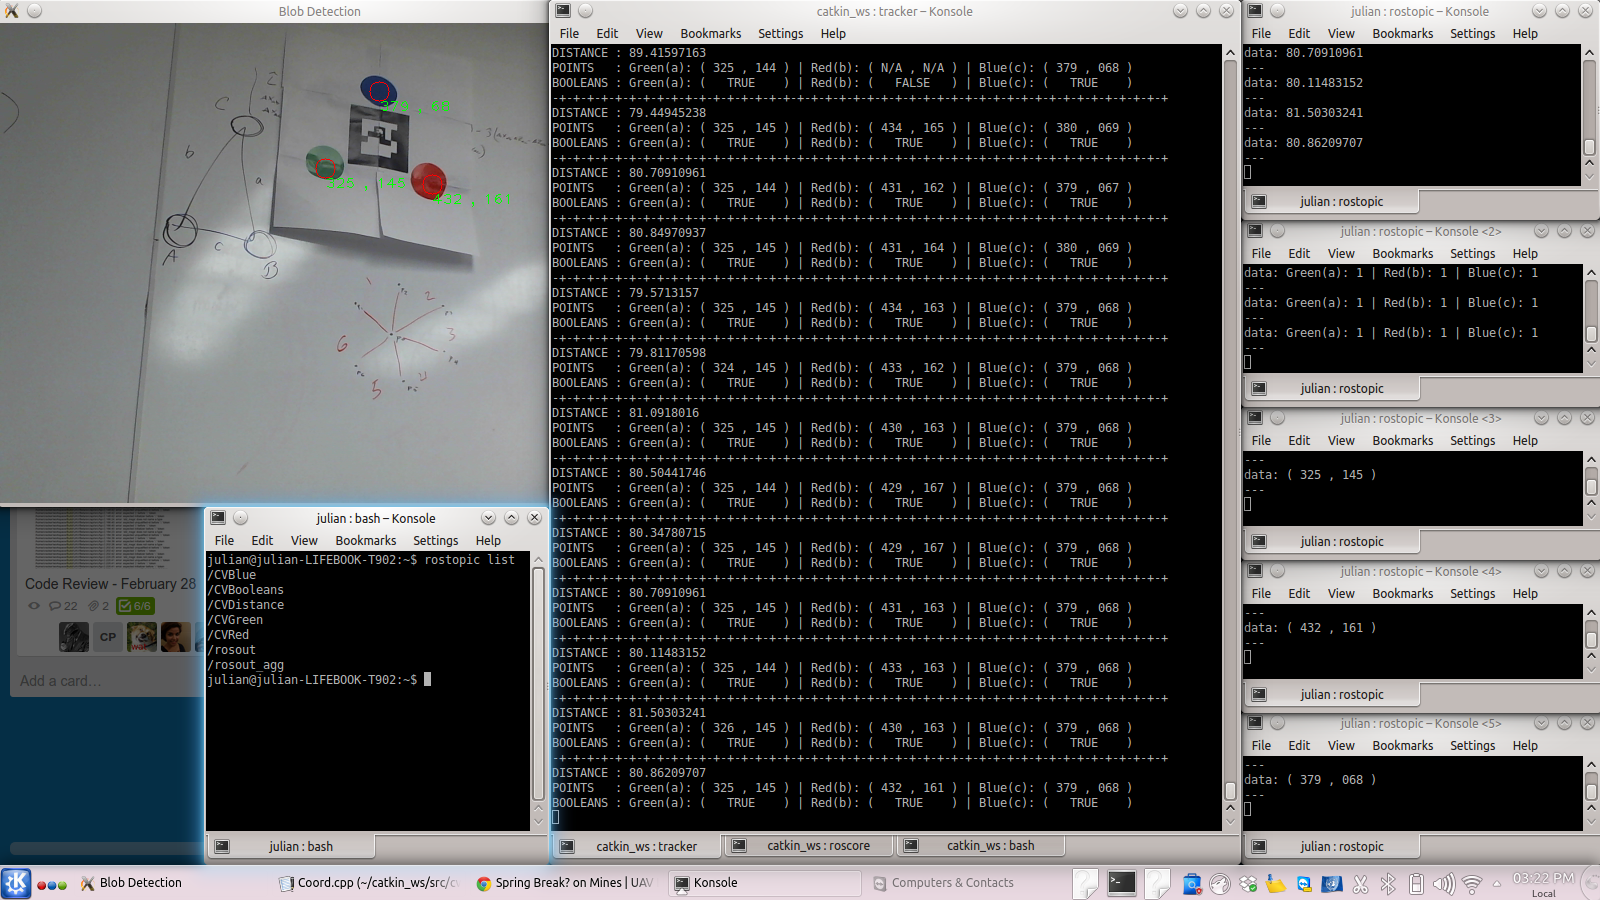
\includegraphics[width=1\textwidth]{resources/img/cv_tracker}
	\end{center}
	\caption{cv\_tracker tracking three coloured circles in the Mobile Computing Lab. \label{cvtracker}}
\end{figure}


\subsection{Technologies  Used}
The object detection and recognition functions for cv\_tracker were written using OpenCV, and the AR tracking is done through the ROS package ar\_track\_alvar.

\subsection{Component  Overview}
\begin{itemize}
 	\item cv\_tracker
	\begin{itemize}
		\item[] custom OpenCV ROS node designed by Julian Brackins and Alex Wulff. Handles craft landing by determining UAV's distance from landing pad based on specified object detection.
	\end{itemize}
 	\item ar\_track\_alvar
	\begin{itemize}
		\item[] Existing ROS package integrated into our project by Hafiza Farzami. Handles craft landing and orientation by identifying and tracking the pose of AR tags.
	\end{itemize}
\end{itemize}

\subsection{Phase Overview}

\subsubsection{cv\_tracker}\label{cvtracker}
The cv\_tracker ros package started out in earlier phases of the Landing Pad project as a proof of concept for identifying object distance using QR Codes. In a camera's video feed, a given subject will appear to be smaller as the camera moves away from that object. Conversely, the item will appear larger the closer the camera is. While this concept is a trivial observation, this change in object size can be utilized to determine the object's current distance from the camera as long as there is prior knowledge of the object's intended size.


A given object's current distance from a camera is the camera's focal length divided by the object's current pixel size from the camera feed, multiplied by the object's original distance. This is expressed in the following equation:

\begin{equation}
	d_{k}'  = w_{k} \times \frac{f}{w_{a}'}
\end{equation}

where:
\begin{itemize}
	\item \begin{math}w_{k} =\end{math} The object's Known Width\footnote{The equation only deals with one dimension of an object's size. One could use height rather than width as long as consistency is maintained in the rest of the calculations.} in meters.
	\item \begin{math}d_{k} =\end{math} The object's Known Distance in meters.
	\item \begin{math}d_{k}' =\end{math} The change in the object's Distance in meters.
	\item \begin{math}w_{a} =\end{math} The object's Apparent Width in pixels. This is simply the object's current width within the video feed coordinate plane.
	\item \begin{math}f=\end{math} The camera's focal length in pixels. The focal length is a measure of how strongly the camera converges or diverges light.
\end{itemize}

In order to calculate the change in distance, or \begin{math}d_{k}\end{math}, the camera's focal length must first be determined using the following formula: 

\begin{equation}
	f = w_{a} \times ( \frac{d_{k}}{w_{k}} )
\end{equation}

The original design in Sprint 2 focused on determining the distance from a QR code by measuring the width of the tag and determining the distance based on the change in size of the code. By Sprint 3, this concept was revised to track coloured circles, arranged in a triangular pattern. This pattern is intended to be implemented as the design for the landing pad. The three coloured circles will be utilized to determine the distance from the landing pad in a similar fashion to the QR code. 

With the three coloured circles, an additional layer of redundancy is incorporated into the tracking routine to ensure accurate distance readings. The triangular pattern allows the tracking software to be later improved to allow the UAV to approach the landing pad from a specific configuration. This functionality would come in to play when integrating a charger to the landing pad, which would facilitate autonomous UAV battery recharge upon landing.

\begin{figure}[tbh]
\begin{center}
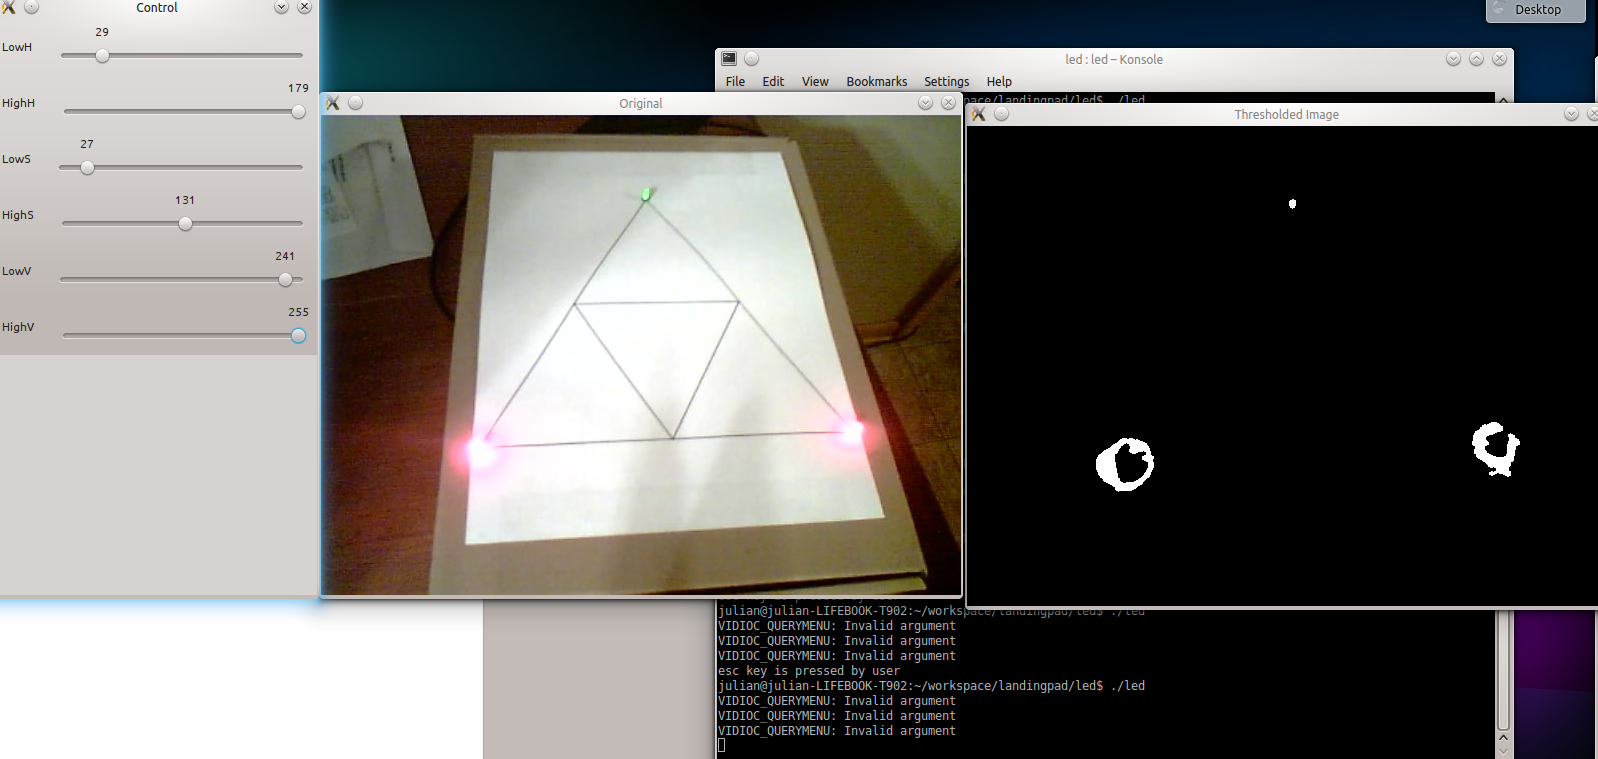
\includegraphics[width=1\textwidth]{resources/img/ledtracking01}
\end{center}
\caption{Early cv\_tracker proof-of-concept using LEDs showing inconsistent color tracking.
\label{ledtracking}}
\end{figure}




\subsubsection{ar\_track\_alvar}\label{artrackalvar}

\begin{figure}[h]
\begin{center}

\includegraphics[width=.30\textwidth]{resources/img/ar_tag_01}
\end{center}
\caption{An AR Tag.
\label{ar}}
\end{figure}

As a way for the UAV to determine the distance away from the UGV and land with the appropriate roll, pitch, and yaw orientation. After Hafiza Farzami joined the team during Sprint 4, the ROS AR tag tracking technology offered by ar\_track\_alvar was incorporated into the craft orientation and landing procedure to be used in conjunction with cv\_tracker in order to provide two separate distance determination methods. The main functionalities of this package used by this project are as follows:

\begin{itemize}
	\item Generating AR tags of different size, resolution, and data encoding
	\item Identifying and tracking the pose of individual AR tags
\end{itemize}

Various colors were experimented with to determine the highest accuracy and the best combination of colors that could be detected from a distance. Ultimately, it was concluded that the black and white AR tags yielded the best results.

%
%\subsection{ Architecture  Diagram}
%It is important to build and maintain an architecture diagram.  However, it may 
%be that a component is best described visually with a data flow diagram. 
%
%
%\subsection{Data Flow Diagram}
%It is important to build and maintain a data flow diagram.  However, it may be 
%that a component is best described visually with an architecture diagram. 


\subsection{Design Details}
\subsubsection{cv\_tracker}
The cv\_tracker ROS package currently publishes the following topics:
\begin{itemize}
	\item  /CVDistance - this displays the distance from the camera to the landing pad in centimeters.
	\item /CVBooleans - displays the tracking state of the circles. true = colour is being tracked. false = colour is not being tracked.
           \item /CVCam - video feed from the camera with the drawn circles to indicate an object is being tracked.
	\item /CVPoints - displays the (x,y) coordinates of the colored objects being detected. The (x,y) are from the camera feed plane.
\end{itemize}
These topics should provide adequate data to the control panel and API in order to issue specified commands for reorienting the UAV for successful landing.


\subsubsection{ar\_track\_alvar}


After initializing ROS using roscore and launching the camera, ar\_track\_alvar publishes the ar\_pose\_marker topic, which contains information about the tag it is detecting as well as a pose message regarding the tag. The pose message contains a point (x,y,z) and a quaternion (x,y,z,w). The quaternion values are converted into roll, pitch and yaw for the control panel display. Figure~\ref{arposemarker} displays the ar\_pose\_marker topic output.


\begin{figure}[tbh]
\begin{center}
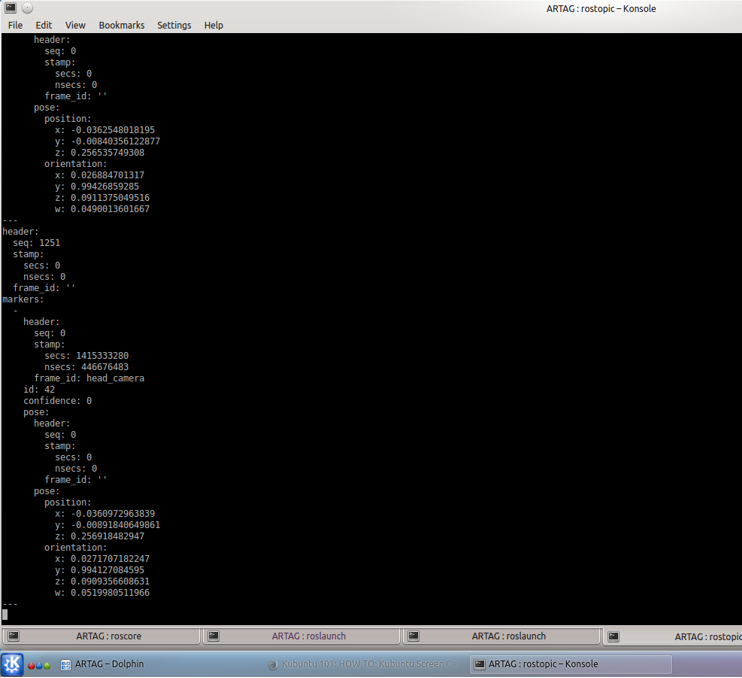
\includegraphics[width=1\textwidth]{resources/img/ar_pose_marker}
\end{center}
\caption{Snapshot of the ar\_pose\_marker topic
\label{arposemarker}}
\end{figure}



\section{Software: Path Planning }\label{softwarepathplanning}

\subsection{Technologies  Used}
The path planning is performed by using the Wavefront algorithm, and the obstacle detection is done by reading in point cloud data.

\subsection{Component  Overview}
The Wavefront algorithm utilizes GPS information processed by ROS. The GPS is located on the UAV, so the waypoints are sent to the UGV through message passing. Due to budget constraints, only one GPS is present, which is simply shared by the ground vehicle and air vehicle since the ground vehicle will only require GPS waypoints while it is moving. At this point in time, the UAV should be situated on the landing pad attached to the UGV.

Point cloud data is generated using the Asus Xtion.

\subsection{Phase Overview}
During Sprints 4 and 5, Samuell Carroll has been utilizing the Asus Xtion, a professional motion sensor for generating point cloud. Using the program PCL-ROS, the Xtion can take in a point cloud image from a ROS topic and output the information as human readable data in a 640x480 lines of 3 float values and an 11 line header. Skipping the header and first 153,600 lines, the numbers are read in, with each set of three being a specific (x,y,z) point in the cloud. The coordinate plane is measured straight ahead from the Xtion in meters. 

The object avoidance routine looks at a minimum distance of 4 meters and anything within that range of the is flagged as a trouble zone for the next image sweep to investigate. Unless the trouble zone was an anomaly, the second sweep will verify the approaching obstacle. If this occurs, the avoidance routine will compare the plane of the object to the drive plane. If the angle between the planes is greater than a given angle, the vehicle will attempt to maneuver around the obstacle. Because the data is being read from a file, the detection code is currently running at a slower rate than originally anticipated. The object avoidance group has been investigating PCL libraries to take the point cloud data and stream the x, y, z coordinates from a ROS topic to streamline the runtime for the object detection routine.

The current object avoidance component can read in 6MB of point cloud data, parse and start looking for objects in approximately 0.5 seconds. Without the files, the team anticipates processing time to be reduced to approximately 0.1 seconds.

%\subsection{ Architecture  Diagram}
%It is important to build and maintain an architecture diagram.  However, it may 
%be that a component is best described visually with a data flow diagram. 
%
%
%\subsection{Data Flow Diagram}
%It is important to build and maintain a data flow diagram.  However, it may be 
%that a component is best described visually with an architecture diagram. 


\subsection{Design Details}

\subsubsection{Navigation Design}
The following code segment details how the wavefront algorithm is used by the ground vehicle, written by Charles Parsons. The UGV performs the wavefront algorithm to fill in values that represent steps from the goal. It starts out by marking the row and column that the goal is represented in, then iterates through the remaining rows using the value from the goal's column as the "seed" value. The algorithm stops evaluating the values once it reaches the starting location. At this point, the path from the starting position and the goal has been established. 
\begin{lstlisting}
void wavefrontFill(int row, int col, int** &map)
{
    int i, j;
    bool goal_found = false;
    int goal_index[2] = {0}; //index 0 = i, index 1 = j
    bool start_found = false;
    int start_location[2] = {0};

    //find the indexes of the goal
    for(i = 0; i < row && !goal_found; ++i)
    {
        for(j = 0; j < col && !goal_found; ++j)
        {
            if(map[i][j] == -1)
            {
                goal_found = true;
                goal_index[0] = i;
                goal_index[1] = j;
            }
        }
    }

    //mark the row and column of the goal with their values
    for(j = goal_index[1] - 1; j >= 0; --j)
    {
        if(map[goal_index[0]][j + 1] == -1)
        {
            map[goal_index[0]][j] = 1;
        }
        else if(map[goal_index[0]][j] == 0)
        {
            map[goal_index[0]][j] = map[goal_index[0]][j + 1] + 1;
        }
    }
    for(j = goal_index[1] + 1; j < col; ++j)
    {
        if(map[goal_index[0]][j - 1] == -1)
        {
            map[goal_index[0]][j] = 1;
        }
        else if(map[goal_index[0]][j] == 0)
        {
            map[goal_index[0]][j] = map[goal_index[0]][j - 1] + 1;
        }
    }
    for(i = goal_index[0] - 1; i >= 0; --i)
    {
        if(map[i + 1][goal_index[1]] == -1)
        {
            map[i][goal_index[1]] = 1;
        }
        else if(map[i][goal_index[1]] == 0)
        {
            map[i][goal_index[1]] = map[i + 1][goal_index[1]] + 1;
        }
    }
    for(i = goal_index[0] + 1; i < row; ++i)
    {
        if(map[i - 1][goal_index[1]] == -1)
        {
            map[i][goal_index[1]] = 1;
        }
        else if(map[i][goal_index[1]] == 0)
        {
            map[i][goal_index[1]] = map[i - 1][goal_index[1]] + 1;
        }
    }
    //mark the rest of the rows and columns using the already marked ones as
    //seed values

    for(i = 0; i < row; ++i)
    {
        start_found = false;
        //skip the row that the goal is on
        if(i != goal_index[0])
        {
            for(j = goal_index[1] - 1; j >= 0 && !start_found; --j)
            {
                if(map[i][j] == 0)
                {
                    map[i][j] = map[i][j + 1] + 1;
                }
                else if(map[i][j] == -2)
                {
                    start_found = true;
                    start_location[0] = i;
                    start_location[1] = j;
                }
            }
            start_found = false;
            for(j = goal_index[1] + 1; j < col && !start_found; ++j)
            {
                if(map[i][j] == 0)
                {
                    map[i][j] = map[i][j - 1] + 1;
                }
                else if(map[i][j] == -2)
                {
                    start_found = true;
                    start_location[0] = i;
                    start_location[1] = j;
                }
            }
        }
    }
    for(j = start_location[1] + 1; j < col; ++j)
    {
        if(map[start_location[0]][j] == 0)
        {
            if(map[start_location[0] - 1][j] < map[start_location[0] + 1][j])
            {
                map[start_location[0]][j] = map[start_location[0] - 1][j] + 1;
            }
            else
            {
                map[start_location[0]][j] = map[start_location[0] + 1][j] + 1;
            }
        }
    }
    for(j = start_location[1] - 1; j >= 0; --j)
    {
        if(map[start_location[0]][j] == 0)
        {
            if(map[start_location[0] - 1][j] < map[start_location[0] + 1][j])
            {
                map[start_location[0]][j] = map[start_location[0] - 1][j] + 1;
            }
            else
            {
                map[start_location[0]][j] = map[start_location[0] + 1][j] + 1;
            }
        }
    }
}

\end{lstlisting}


\subsubsection{Obstacle Detection Design}
The following code segment details the findObjects() function written by Saumel Carroll. This function will traverse the image looking for points in a given threshold value. If a point within the threshold, the function will look around the point and try to determine if the point is an object or just an anomaly by flagging trouble spots. If the function decides the point is part of an object, the program will try to find its plane and decide if it is a troublesome object. Troublesome objects are classified as objects within 30 degrees of the drive plane.

\begin{lstlisting}
void findObjects (vector < vector < point > > &image)
{
  int goLeft, goRight = 0;
 // if the object is within the minimum threshold try to find 
 //the object plane
 // do this by taking points around it in the i and j positions and if they 
 //are about the same distance away assume they are the same object
 // start at multiple rows and see if we have any trouble areas save 
 //all trouble
 // i and j zones that we found on the previous sweep and see if the 
 //object is still there, if so 

  int listSize = _lastSweep.size();
  list<rowcol>::iterator lastSweepIter;
  if (listSize > 0)
  {
    for (lastSweepIter = _lastSweep.begin();
           lastSweepIter != _lastSweep.end(); lastSweepIter++)
    {
      if (!scanArea(image, *lastSweepIter, lastSweepIter))
      {
            // remove from our _lastSweep list
             list<rowcol>::iterator tempIter = lastSweepIter;	
             if (!_lastSweep.size() != 1)
	  {
                 lastSweepIter--; 
                 // decrement by one so we don't skip a possible object.
	   }	
          _lastSweep.erase(tempIter);
      }
    }
  }
  
// put in a for loop that scans 8 random rows that aren't equal to each other
// then save the trouble spots (i and j) so we can determine what to do
// If an object is still there avoid if not it moved and keep going
  for (int scannedRows = 0; scannedRows < 30; scannedRows++)
  {
    // scan random rows looking for troubled spots
    int scanRow = rand() % 240; // randomly choose a row from 0-239
    scanRows (image, scanRow, goLeft, goRight); // scan that row
  }
// add all elements from _currSweep to _lastSweep
  _lastSweep.splice(_lastSweep.end(), _currSweep); 
  _currSweep.clear(); // ensure _currSweep is empty
}
\end{lstlisting}

\section{Software: Control Panel }\label{softwarecontrolpanel}

\subsection{Technologies  Used}
The control panel is a top level graphical user interface written in C++ using Qt. Underneath the graphical layer, the control panel utilizes ROS to read and send data to ROS topics.

\subsection{Component  Overview}
The following is a list of features the Control Panel is capable of performing:
\begin{itemize}
	\item Displays the (x, y) coordinates of the Red, Green, and Blue blobs located on the landing pad.
	\item Subscribes to the ar\_pose\_marker topic form AR tags and displays (x, y, z) from the UAV to the landing pad on the UGV in the "Position" field. Quarternion values are also calculated from the AR tags, giving the roll, pitch and yaw data from the aircraft.
	\item Subscribes to the GPS node in the UAV and displays the latitude, longitude, and altitude.
	\item Displays whether or not the control panel is connected and running, confirms whether or not a joystick is connected to the computer running the control panel, and displays the height of the UAV in relation to the landing pad.
\end{itemize}

\subsection{Phase Overview}
The control panel is a centralized tool where it displays all the sensor data and is able to control the UGV via the computer keyboard or a USB Playstation 3 controller.
The control panel was initially built by Matt Richard and Scott Logan. This semester, Hafiza Farzami added additional functionality for our project. For instance, the blob detection data, the AR tag data, and distance display have been integrated into the control panel to display the relevant data for the ground vehicle and air vehicle. The GUI and the new ROS nodes for subscribing to the topics published from the new nodes and displaying them on control panel were written and integrated into the existing control panel system.


\subsection{Design Details}
Figure~\ref{ctrlpanel} displays the control panel after the modifications had been made to it this semester.

\begin{figure}[tbh]
\begin{center}
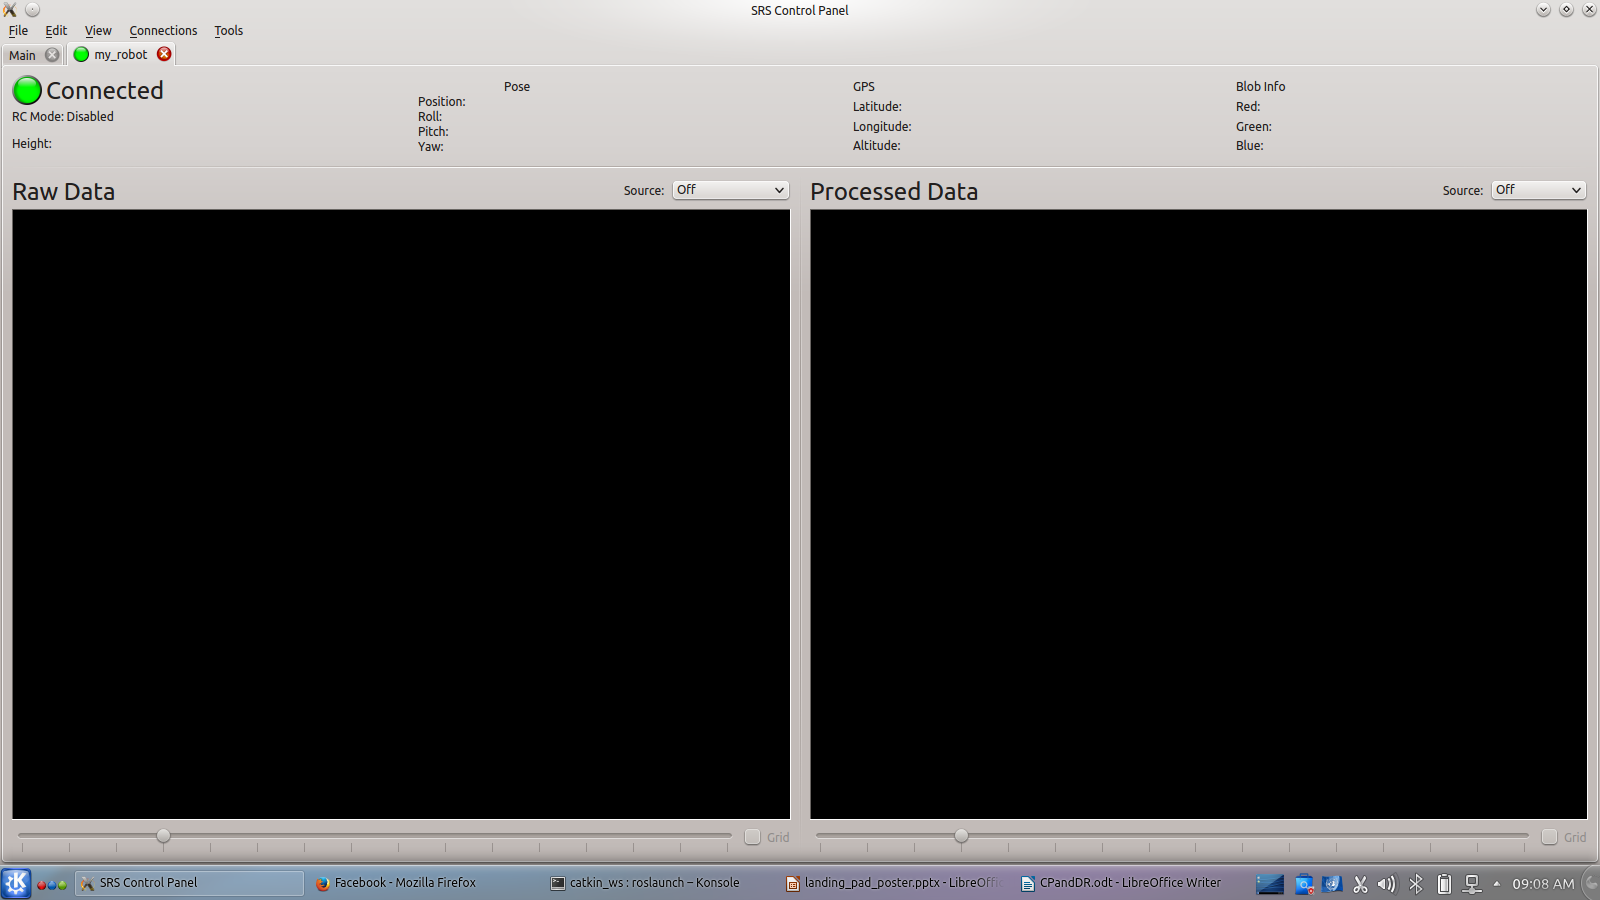
\includegraphics[width=.5\textwidth]{resources/img/control_panel}
\end{center}
\caption{Customized Control Panel.\label{ctrlpanel}}
\end{figure}


\section{Drive System }\label{drivesystem}

\subsection{Technologies  Used}
The drive system uses the Ackerman Steering system, and is based off the skid\_steer drive, a differential drive node written by former SDSM\&T student Andrew Pierson. Further details on how the drive system functions are in Section~\ref{drivesystemdesigndetails}.

\subsection{Drive System Diagram}
Figure~\ref{ack_drawing} is an excerpt from Dr. McGough's Introduction to Robotics book detailing how the Ackerman Steering system functions.


\begin{figure}[tbh]
\begin{center}
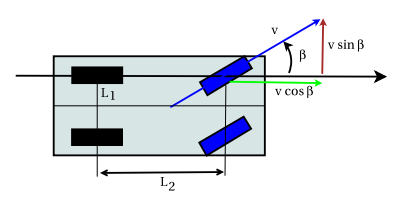
\includegraphics[width=.5\textwidth]{resources/diagram/ackerman_drawing}
\end{center}
\caption{Ackerman Steering System \label{ack_drawing}}
\end{figure}

\subsection{Design Details}\label{drivesystemdesigndetails}
The drive system takes angular and linear velocity inputs from a USB controller and uses the linear equations in Figure~\ref{ack_equation} to send the velocity values to the back wheels through the motor controller attached to the back wheels. The turning angle values is sent to the front wheels through the front motor controller.

\begin{figure}[tbh]
\begin{center}
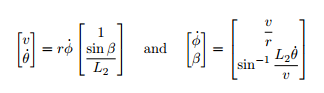
\includegraphics[width=.5\textwidth]{resources/diagram/ackerman_equation}
\end{center}
\caption{Ackerman Steering Formula \label{ack_equation}}
\end{figure}

\section{UAV }\label{uav}

%\subsection{Technologies  Used}

\subsection{Component  Overview}
The following subsection details the components onboard the current UAV:
  \begin{itemize}
    \item AMP 2.6 - flight control board
    \item 3dr ublox GPS with Compass - compass and gps
    \item R5800X receiver and TXV582 - video transmitting
    \item Sony HAD 520 line camera - on board camera
    \item Spektrum AR7000 - 7 channel receiver
    \item 915 MHz radio - telemetry with ground station
  \end{itemize}


\subsection{Phase Overview}
The Phase Overview for the UAV will be broken up into the different progress reports returned throughout the project timeline.

\begin{itemize}
\item Sprint 2 

The quadcopter used for research and development during the landing pad project was a device inherited by our team from the UAV team at the South Dakota School of Mines and Technology. As a result, there were a number of repairs required to perform before the UAV was in working condition. During Sprint 2, 2 new batteries and battery adapters as well as a new Electronic Speed Controller were purchased in order to get the quad rotor working for testing in later sprints.

\item Sprint 4

By Sprint 4, the first person view camera was set up, allowing video to be streamed from the aerial vehicle to a ground computer. Autonomous flight was also implemented at this time by changing settings on the UAV controller. The vehicle is now able to switch from transmitter control to autonomous control.

\item Sprint 5

Using the ROS package Mavros, a user is now able to send commands to the UAV using ROS. by connecting the UAV to a flight control board, a user is able to issue commands to the UAV by sending the vehicle a list of waypoints to navigate. Using the onboard telemetry unit, the UAV is able to wirelessly link to a ground computer within a mile range.
\end{itemize}

%\subsection{ Architecture  Diagram}
%It is important to build and maintain an architecture diagram.  However, it may 
%be that a component is best described visually with a data flow diagram. 
%
%
%\subsection{Data Flow Diagram}
%It is important to build and maintain a data flow diagram.  However, it may be 
%that a component is best described visually with an architecture diagram. 


\subsection{Design Details}
Roscopter is a ROS interface designed for Arducopter utilizing the Mavlink 1.0 interface~\cite{roscopter}.

The package publishes various sensor topics that our custom API and control panel can monitor:
\begin{itemize}
	\item /attitude - imu information
	\item /gps - gps
	\item /rc - value of current raw rc input
	\item /state - displays whether the uav is armed or not
	\item /vfr\_hud - airspeed, ground speed, heading, throttle, alt, climb
\end{itemize}

UAV control instructions can be sent to a vehicle running Roscopter by publishing to /send\_rc topic. This topic reads in raw RC channel values between 1000-2000 and uses these values to override the values given from an RC controller.


\section{UGV }\label{ugv}

\subsection{Component  Overview}
The following components interface with the UGV. Please refer to each specified component's design section for additional details
\begin{itemize}
	\item Custom API - The ground vehicle, just like the UAV, uses the custom API designed by Alex Wulff detailed in Section~\ref{softwarecustomapi}
	\item Drive System - an Ackerman-based rear drive system detailed in Section~\ref{drivesystem}
	\item Path Planning and Object using Stereo vision - Section~\ref{softwarepathplanning}
\end{itemize}


\subsection{Phase Overview}
The Phase Overview for the UGV will be broken up into the different progress reports returned throughout the project timeline.

\begin{itemize}
\item Sprint 3

By the end of Sprint 3, the frame design for the ground vehicle had been completed, with the intention to start building the vehicle before Sprint 4. At this time, a front-end steering system from a golf cart was purchased for use as the UGV drive system.

\item Sprint 4

Under the supervision of Alex Wulff, the UGV designs reached completion, incorporating the front differential acquired from the golf steering system. The external frame is nearly complete; the design requires additional support gussets and a connection to the power supply and landing pad.

\item Sprint 5

During Sprint 5, Alex Wulff mounted the steering system to the frame and attached the motors, motor controls and tires to the frame. The drive wheels still need to be secured to ensure slip does not occur while propelling the vehicle and to create a better gear interface with the Ackerman differential.

\item Sprint 6

During Sprint 6, the worm gear used for controlling the steering system via a motor was installed using a bracket which secured the motor drive in place. Wiring the motor controls was done by Samuel Carroll, and Hafiza Farzami worked on the motor controls for the drive system. On the way to the design fair, the bracket securing the motor for the drive system was shifted out of alignment. A new, more rigid bracket will need to be installed in order to facilitate steering for the ground vehicle in the future.

\end{itemize}
